\documentclass[10pt,conference]{IEEEtran}
\IEEEoverridecommandlockouts

\usepackage{amssymb,amsmath,color,amsbsy}
\usepackage{subfigure}
%\usepackage{subcaption}
\usepackage{cite}
\usepackage{algorithm}
\usepackage{algorithmic}
\usepackage{amsfonts}
\usepackage{amssymb}
\usepackage{graphicx}
\usepackage{epstopdf}
\usepackage{leftidx}
\usepackage{dsfont}
\usepackage{url}
\usepackage{amsmath}
%\usepackage{bbm}
%\usepackage{mathrsfs}
%\usepackage{xcolor}

\newcommand{\ie}{\emph{i.e., }}
\newcommand{\eg}{\emph{e.g., }}

%\newcommand{\Pr}{\mathrm{Pr}}
\newcommand{\Children}{\textsf{Children}}
\newcommand{\Parent}{\textsf{Parent}}
\newcommand{\Decoder}{\textsf{Decoder}}
\newcommand{\Range}{\textsf{Range}}
\newcommand{\Interval}{\textsf{Int}}

\ifodd 1
\newcommand{\rev}[1]{{\color{blue}#1}}
\newcommand{\com}[1]{\textbf{\color{red}  #1}}
\newcommand{\res}[1]{\textbf{\color{magenta} (RESPONSE: #1)}}
\newcommand{\del}[1]{}

\newcommand{\xiaohong}[1]{\textcolor{blue}{#1}}
\newcommand{\yc}[1]{\textcolor{red}{#1}}
\else
\newcommand{\rev}[1]{#1}
\newcommand{\com}[1]{}
\newcommand{\res}[1]{}
\newcommand{\del}[1]{}
\fi

\setlength{\floatsep} {0pt } \setlength{\textfloatsep} {0pt plus 1pt minus 2pt}
\setlength{\abovecaptionskip}{0pt} \setlength{\belowcaptionskip}{0pt}

\title{Verification on Out-of-date Radiomap Against Environment Impacts}
\author{\IEEEauthorblockN{Zhiqi Yang, Yongcai Wang, Lei Song}
\IEEEauthorblockA{Institute for Interdisciplinary Information Sciences (IIIS), Tsinghua University, Beijing, P.R.China, 100084\\
Email: wangyc@tsinghua.edu.cn}
}
%\date{}   
\begin{document}         
\maketitle                     % Activate to display a given date or no date
\begin{abstract}
In a number of indoor positioning techniques, received signal signatures (RSS) has been widely used. Among them, path-loss model and radiomap linear regression-based model is put forward to estimate locations. The path-loss model uses logarithmic dB linear formula to estimate RSS transmitting loss, while the radiomap model usually contains offline coefficients training and online locating. Path-loss model only performs well in free space, while radiomap model often becomes outdated when facing environmental chagnes. In this paper, we design a novel experimental system to verify these models, the devices contain Android devices and Raspberry Pi, the Raspberry Pi is cheap and easy to configure, particularly, the Raspberry Pis are programmable and configurable based on linux, which made it possible to act as both transmitters and receivers, thus more powerful than wlan APs. Experimental results show the shortage of path-loss model and the radiomap's disability of adaptivity to environmental changes. \yc{Moreover, we put forward a novel online adaptive algorithm to solve the unadaptivity of radiomap model. The simulation shows satisfiable results.} 
\end{abstract}

%-------------------------------------------------------------------------------------------------------------------------------------

\section{Introduction}
Since RADAR \cite{radar}, a radio-frequency based system, was first put forward for indoor positioning, a number of techniques including time-based, angle-based and power-based models come into being. Among these models, power-based stands out because of the better performance on indoor location with obstacles. Specifically, the power-based model make use of received signal signatures as key measurements to estimate distance. Normally there exists two power-based methods: path-loss model and fingerprinting. Path-loss model usually apply log-distance formula to formulate RSS transmitting power, but the model only performs well in free space, while in indoor environments, devices and obstacles are almost everywhere, affecting path-loss model accuracy much. Fingerprinting model contains two phases: offline training phase and online phase. In offline training phase, the transmit and receive power strength are stored as matrix (called radiomap) and then calculate offline coefficients. In online phase, we apply the offline coefficients to the model and calculate the measured location. The biggest problem of fingerprinting model is that it can not adapt to environmental changes, thus making the offline coefficients out of date, besides, the offline calculate process also requires time consuming. In this paper, we introduce a novel system to verify these two models, the system contains regular mobile Android devices, while we use a novel device called Raspberry Pi \cite{raspberry} acted as the wlan AP. The Raspberry Pi is a "micro-computer" that can be plugged into a computer monitor, it's cheap and programmable based on linux. After configuration, it could automatically detect AP around and be detected by others Pis, besides, it's also set to send AP's mac address and corresponding RSS to server for following operation. As Raspberry Pi can also be charged by portable power source, we can adjust the Raspberry Pi's locations to achieve different thoughts, which is far more better and flexible than ordinary experimental static wlan APs. In this paper, we fix Raspberry Pi in different locations and collect RSS data to verify path-loss and fingerprinting models. The paper is organized as follows: part II will introduce the problem models, verification methods and model evaluation, part III will explain how we build the experimental system, part IV will show experimental results, part V is conclusion and future work.
%The verification contains two phases: inter-Raspberry Pi verification phase and radiomap verification case. Both phases contain offline training and online verification. By calculating error between the calculated RSS using offline coefficients and measured RSS, we would come up with the conclusion well: the model cannot adapt to environmental changes.

%-------------------------------------------------------------------------------------------------------------------------------------

\section{Problem Model and Related Work}
Recently, many power-based approaches have been proposed to focus on indoor positioning, we can roughly conclude these solutions into 2 phases, 1) based on model; 2) based on measurement. Model phase solutions usually contain static and dynamic models. Radiomap based on such models \cite{site} consider path-loss model, by applying distance partitioned path-loss model and characterizing RSS signatures, the paper proposed a wall breakpoint model to fulfill the use in indoor environment. But the problem is the model may not be that accurate, it needs specific measurement for environment, moreover, RSS signature collection is expensive and time-consuming, besides, research community has no access to commerce companies' signature databases, making it difficult for model application. Others like \cite{dynamic} consider GPR(Gaussian Process Regression), by building an optimized power profile for each AP, it's able to construct radiomap online and achieve positioning accuracy. But the problem is that once positioning areas become large, the AP number needed for profiling increases immediately, besides, the AP Power Profiling mathematic model using GPR may be a little complex to understand and the kernel function also needs learning. Another solution phase is based on measurement. The measurement phase solutions tend to achieve online adaptive calculating and positioning without using too complex models and focus more on the optimization of experimental system deployment, apply linear-regression model to train offline and predict online. The problem is that simply training offline and applying coefficients online would generally be out-of-date because of the indoor environmental changes.

In this paper, we first build a novel system to verify some typical models' unadaptivity on environmental changes, \yc{then we consider for adaptive solutions.} In the first step, we consider the distance partitioned path-loss model, wall breakpoint model and linear regression model's verification. In the model verification experimental system, novel devices like Raspberry Pi are added in to act as wlan AP. The Raspberry Pi is cheap and easy to move based on mobile battery charging, besides, the built-in linux system makes it easy to program, configure and transplant and copy, which making it possible to perfectly replace wlan AP for indoor positioning experiment and deploy in a large scale without that time consuming.

Similarily, our verification contains two phases: offline training and online verifying. We use our novel system to collect a number of data sets, training set would be used for offline training and obtain coefficients, verification set would be used to verify the effectivity of training coefficients.

For verification convenience, we define SRE(Square Root Error) and AE(Average Error) as the measurement standard to show the environmental change impacts, that is, if the error is bigger than threshold, it means the path-loss model cannot fit well or radiomap model cannot adapt to environmental changes become out-of-date. The SRE and AE is calculated as follows:
$$SRE = \dfrac{\Big\lVert R-R_{cal} \Big\rVert_2}{Time\ Length}, AE = \dfrac{\Big\lVert R-R_{cal} \Big\rVert_1}{Time\ Length}$$
Where:
\begin{itemize}
	\item $R$ represents the measured RSS in verification data set, which is accurate
	\item $R_{cal}$ represents the calculated RSS using training set coefficients
\end{itemize}
In this paper, the to-be-verified radio channel model contains two phases: path-loss model and wall breakpoint model, and the to-be-verified fingerprinting linear regression model contains two phases: inter-Raspberry Pi model and radiomap model.

\subsection{Distance Partitioned Path-Loss Model}
The path-loss model belongs to radio channel model, its basic assumption is that the area between transmitter and receiver is not often homogeneous, so the propagation path-loss gradient from the AP to the receiver is not uniform, not just a single distance-power gradient, and in this simplified model the propagation path is partitioned into two sections using a breakpoint distance parameter $d_{bp}$, each section uses a separate distance-power gradient parameter to characterize the path-loss. The formula denotes as follows:

\begin{equation}
{L_p} = \left\{ {\begin{array}{*{20}{l}}
  {{L_0} + 10{\alpha_1}\log (d),{\text{if }}d < {d_{bp}}} \\ 
  {{L_0} + 10{\alpha_1}\log ({d_{bp}}) + 10{\alpha _2}\log \left( {\dfrac{d}{{{d_{bp}}}}} \right),{\text{if }}d > {d_{bp}}} 
\end{array}} \right.
\end{equation}
Where: 
\begin{itemize}
	\item $d$ represents the distance from transmitter to receiver in meters
	\item $L_p$ represents the path-loss over the distance $d$ in $dB$,
	\item $L_0$ represents the path-loss over the first meter in $dB$
	\item $\alpha_1$ and $\alpha_2$ represents separate distance-power gradients sections before and after breakpoint
	\item $d_{bp}$ is the static breakpoint distance in meters. 
\end{itemize}

The model considers different parameters for different distances, in order to verify comprehensively, we can design a Raspberry Pi lay-out. Each Pi can act as both transmitter and receiver, and the inter-distances are set and measured precisely. Using measured RSS we can get $L_p$, by substituting distance in the model, we can get the calculated $L_p$, then we can calculate $SRE$ and $AE$ with measured and calculated $L_p$ value to verify the model.


%-------------------------------------------------------------------------------------------------------------------------------------

\subsection{Wall Breakpoint Model}

Distance factor considers only indoor-to-indoor environment, which assumes that there is not any blocks in the transmitting channel, while in actual indoor buildings, blocks exist and play an important role in RSS transmitting, such as wall block and door block. In [Site-Specific] paper, the wall breakpoint model is described as follows:
\begin{equation}
\footnotesize{
\begin{gathered}
  {L_p} =  \hfill \\
  \left\{ {\begin{array}{*{20}{l}}
  {{\!\!L_0}\!\!+\!\!10{\alpha _1}\log ({d_{wbp}})\!\!+\!\!10{\alpha _E}\log \left( {\dfrac{d}{{{d_{wbp}}}}} \right)\!\!+\!\!{L_W},{\text{if }}{d_{bp}}\!\!>\!\!{d_{wbp}}} \\ 
  {{L_0}\!\!+\!\!10{\alpha _1}\log ({d_{bp}})\!\!+\!\!10{\alpha _2}\log \left( {\dfrac{{{d_{wbp}}}}{{{d_{bp}}}}} \right)\!\!+\!\!10{\alpha _E}\log \left( {\dfrac{d}{{{d_{wbp}}}}} \right)\!\!+\!\!{L_W},{\text{if }}d\!\!>\!\!{d_{bp}}} 
\end{array}} \right. \hfill \\ 
\end{gathered}
} 
\end{equation}

Where  the added parameters are:
\begin{itemize}
	\item $d_{wbp}$ represents the dynamic AP specific wall breakpoint defined by the distance from the AP to the exterior wall of the building in meters
	\item $\alpha_E$ represents the distance-power gradient for the exterior path
	\item $L_w$ is the path-loss for the exterior wall in $dB$
\end{itemize}

$d_{wbp}$ is a dynamic variable distance from AP to exterior wall. In this model verification, we only need to add a wall in, and arrange Raspberry Pi inside and outside the wall. The verification step is similar as path-loss model, we also use $SRE$ and $AE$ to measure the model's accuracy.

%-------------------------------------------------------------------------------------------------------------------------------------

% ------------draw Inter-Raspberry Pi Model & Radiomap Model
\begin{figure*}[htbp]
%\centering
\begin{minipage}[t]{0.5\textwidth}
	\centering
	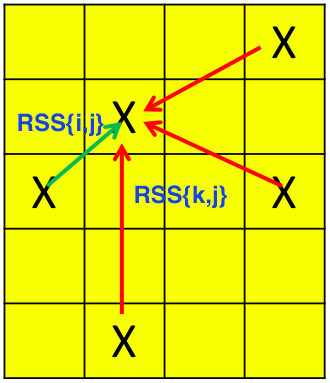
\includegraphics[scale=0.3]{model1}
	\caption{(simplified) Inter-Raspberry Pi Model}\label{inter}
\end{minipage}
\begin{minipage}[t]{0.5\textwidth}
	\centering
	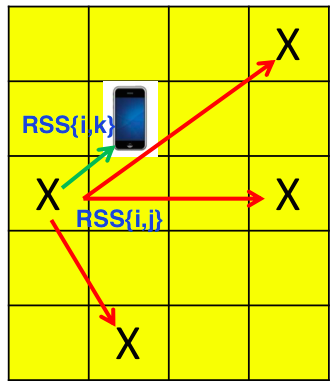
\includegraphics[scale=0.3]{model2}
	\caption{(simplified) Radiomap Model}\label{radiomap}
\end{minipage}
\end{figure*}

\subsection{Inter-Raspberry Pi Model}

The Raspberry Pis are configured so that each Pi can detect wlan AP RSS around and be able to be detected by other Pis. Applying the linear regression model, we can denote as follows:
$$RSS_{i,j}=\sum_{k\neq i, k\neq j}^m\alpha_{i,k,j}RSS_{k,j}+const.$$
Where: 
\begin{itemize}
	\item $RSS_{i,j}$ represents Raspberry Pi ID $i$'s RSS detected by Raspberry Pi ID $j$
	\item $m$ is the number of Raspberry Pi
\end{itemize}

The equation indicates that a Pi $i$'s RSS detected by location Pi $j$ can be linear represented by other Pis' RSS detected by location Pi $j$. And this is one moment. If we unit a long time series of detected RSS and denote in matrix style as follows: \\

$\begin{bmatrix}
R_{i,j}^1 \\
. \\
R_{i,j}^t  \\
\end{bmatrix}$ = 
$\begin{bmatrix}
R_{1,j}^1 & R_{2,j}^1 & ... & R_{m,1}^1 & 1 \\
. \\
R_{1,j}^t & R_{2,j}^t & ... & R_{m,1}^t & 1 \\
\end{bmatrix}$  
$\begin{bmatrix}
\alpha_{i,1,j} \\
. \\
\alpha_{i,m-1,j} \\
\end{bmatrix}$  \\
we can simplify the matrix form as $\bold{R=A\alpha}$, \\
Where: 
\begin{itemize}
	\item $t$ is offline training time length
	\item $\bold{\alpha}$ is offline training coefficients.
	\item $\bold{R}$ is the left measured RSS matrix
	\item $\bold{A}$ is the right matrix linear representation
\end{itemize}

Using least square method we can calculate offline efficients as follows:
$$\bold{\alpha=(A^TA)^{-1}A^TR}$$

After calculating offline efficients, we then collect new data $\bold{R' \& A'}$ and compare measured RSS $\bold{R'}$ with calculated RSS $\bold{R_{cal}}$, where $\bold{R_{cal}=A'\alpha}$. Then we use SRE and AE as the measurement standard.

%-------------------------------------------------------------------------------------------------------------------------------------

\subsection{Radiomap Model}

In the radiomap model, android devices join in. We develop an app called $\textit{Wiloclient}$, the app can detect the AP around and send to server automatically. Applying the linear regression model, we can denote as follows:
$$RSS_{i,k}=\sum_{j=1,j\neq i}^m\beta_{i,j,k}RSS_{i,j}+const.$$

Where:
\begin{itemize}
	\item $RSS_{i,k}$ represents Raspberry Pi ID $i$'s RSS detected by mobile devices at location $k$
	\item $RSS_{i,j}$ and $m$ represents the same in Inter-Raspberry Pi model
\end{itemize}

The equation indicates that a Pi $i$'s RSS detected by mobile device in location $k$ can be linear represented by Pi $i$'s RSS detected by other Pis. Similarily, we unit a long time series of detected RSS as offlinet training time length and denote as follows: \\

$\begin{bmatrix}
R_{i,k}^1 \\
. \\
R_{i,k}^t  \\
\end{bmatrix}$ = 
$\begin{bmatrix}
R_{i,1}^1 & R_{i,2}^1 & ... & R_{i,m}^1 & 1 \\
. \\
R_{i,1}^t & R_{i,2}^t & ... & R_{i,m}^t & 1 \\
\end{bmatrix}$  
$\begin{bmatrix}
\beta_{i,1,k} \\
. \\
\beta_{i,m,k} \\
\end{bmatrix}$  \\

We can also simplify the matrix form as $\bold{R=B\beta}$, and using least square method we can calculate offline efficients as follows:
$$\bold{\beta=(B^TB)^{-1}B^TR}$$

Similarily we verify the model using SRE and AE as the measurement standard. The two simplified model map is shown as Fig. \ref{inter} and Fig. \ref{radiomap}.

\subsection{Conclusion}
The path-loss model is a traditional RSS model for indoor localization, in \cite{site}, they considered the wall effect and add a dynmaic site-specific wall breakpoint model in. These models are usually logarithmic dB linear based model, the formula is easy to understand and calculate, but the disadvantages are also obvious: 1) First, the formula is rough, path-loss model mainly acts well in free space, the propagation path-loss gradient is partitioned into two sections, which means it does not satisfy many other environments, while although wall breakpoint model adds wall effect in, the variable $d_{wbp}$ is dynamic and has to consider the specific wall distance from AP, which means it's not dynamic and adaptive; 2) Second, the gradient section number is difficult to choose because it is much affected by environment dynamic changes; 3) Third, the parameters such as $\alpha_1$ also depends on the environment measurements, some like $d_{bp}$ is even relative to base and mobile station antennas's height and carrrier frequency's wavelength \cite{wireless}, making the paramenters dynamic and hard to measure.

Therefore, more interests focus on radiomap model. Since it considers offline training, the parameter measurement is automatic, while online we only need to apply these offline parameters to formula and calculate the estimated RSS. But there are two main problems: 1) the offline training is usually time consuming, in order to train precise parameters, we have to apply a number of data, which means low efficiency; 2) the parameters cannot adapt to environmental changes, even if we get the parameters in offline step, they may become out-dated in online because of environment change effects, the effect is especially obvious in linear regression model.

In this paper, we will build a novel system to verify these models' unadaptivity and put forward an improved linear adaptive model.

%-------------------------------------------------------------------------------------------------------------------------------------

\section{Measurement System}
Our experiment environment lies in the third floor of MMW building in Tsinghua, the lay out is shown as Fig. \ref{layout}, the area is 922 $m^2$ and contains a corridor and a number of rooms with different size. We will place our hardware and software in this area to do experiments and collect data.

%\DeclareGraphicsExtensions{.eps,.mps,.pdf,.jpg,.png}
\begin{figure*}[htbp]
\centering
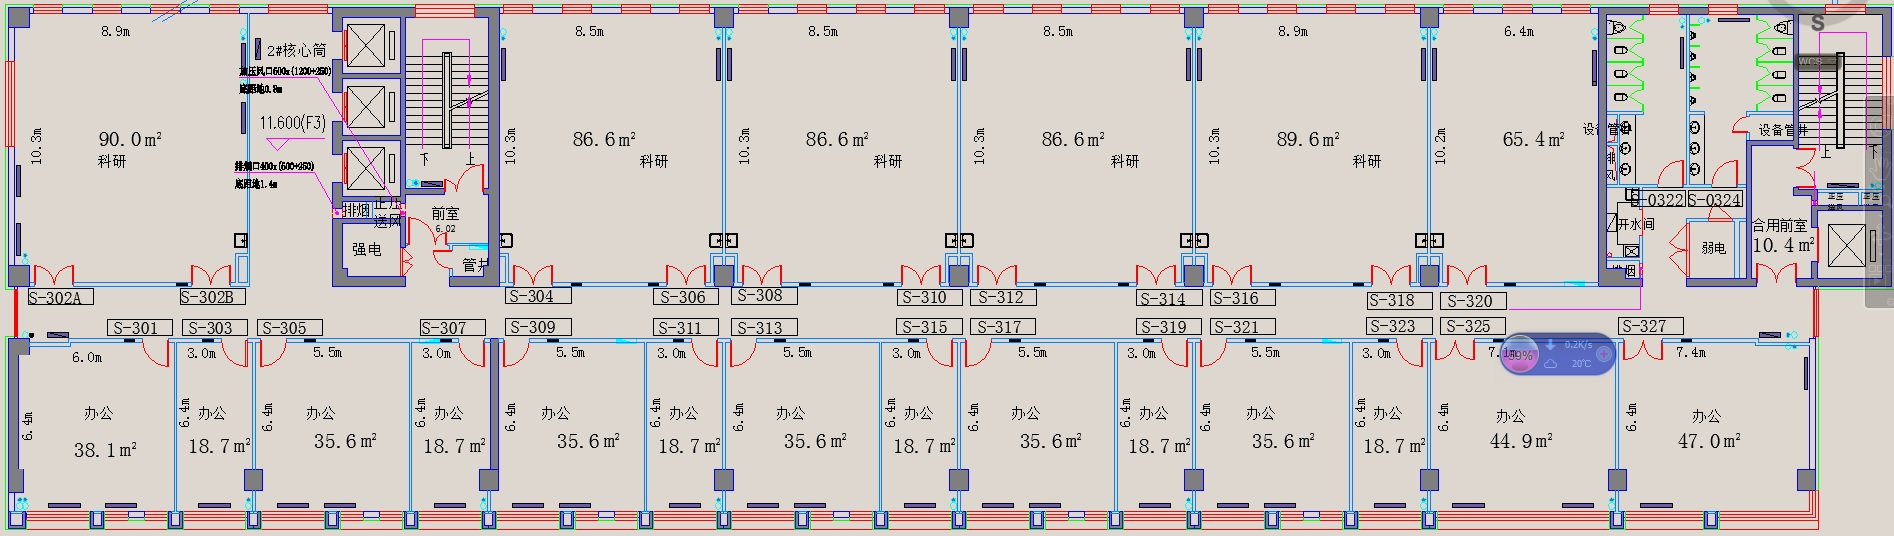
\includegraphics[scale=.3]{3floor} 
\caption{Experiment Environment Layout}\label{layout}
%label must write behind caption, in same line!!
\end{figure*}

\subsection{Hardware}
Our hardware contains a router, a number of Raspberry Pis, PC server, Android mobile devices such as Nexus 5 and Tablet. 

\subsubsection{Raspberry Pi configuration}
Each Raspberry Pi possesses two network cards, one to be configuraed as AP so that it can detect APs' RSS nearby and be detected by others, which means it can act as both transmitter and receiver. By detecting AP RSS, the Raspberry Pi would send data to server, the data segment format is optimized with Raspberry Pi ID, detecting AP number, AP MAC address and correponding RSS inside. Since Pi ID and AP MAC address are both unique, it would be easy for server to know which AP the data segment belongs to and process data more conveniently and automatically, besides, with the router, the Raspberry Pis can send all data to server for following localization under the same school subnet without any data package loss.
\paragraph{RSS Collection Algorithm in Raspberry Pi}
With a series of simple linux order, the Raspberry Pi can be easily configurated to act as both transmitter and receiver, but that's not enough, to automatically detect APs' RSS nearby and send information to server, we design an RSS collection algorithm employed in Raspberry Pi to detect and collect nearby AP information and send to server. We call the algorithm \textit{NormScore}. 
\yc{TO SONG LEI: Introduce the algorithm in zmqserver.c...} \textit{NormScore}'s main idea focuses on score ranking based on gaussian distribution, that is, the algorithm considers the APs obey gaussian distribution and calculate mean and convariance by collecting all APs' information, then we calculate the probability with current RSS as the input value and add to score, which is the final result.
\paragraph{RSS transmitting protocol in Raspberry Pi}
\yc{TO SONG LEI: Introduce ZeroMQ protocol and its advantages...} \\
After configuration and collection algorithm design, we need to solve data transmitting problem. The transmitting principle is based on an opensource protocol called ZeroMQ protocol \cite{zmq}, which can be used as an intelligent transport layer for distributed apps. Actually, ZeroMQ is so powerful that we only need to make use of some functions and protocols of it. In this paper, we mainly design the data transmitting with the help of ZeroMQ protocol, by making use of the libzmq engine and adapting to our system, we can easily transmitt the data over TCP and avoid re-inventing wheel.
\paragraph{Easy to duplicate}
All configurations store in SD card, once a Raspberry Pi is configurated successfully, we only need to backup its SD card content and copy to other Raspberry Pis with a few simple linux orders in a short time, which makes it possible to achieve large number of Raspberry Pi configuration without too much consuming time.

\subsubsection{Android mobile devices}
The mobile devices include Nexus 5 and Tablet installed with newest Android 4.4 version, by installing an app called $\textit{Wiloclient}$ and setting the option, the device can detect nearby APs' RSS and send to server with APs' Mac Address and RSS. The devices plays an important role in radiomap model verification. Its mobility makes it easy to verify in different locations and path walking simulation.

\subsection{Software}
Our software mainly contains C, MATLAB and Java. Java is used to develop Andorid app, C and MATLAB are made used of dealing with RSS data, present connection, calculating offline coefficients and error.
\subsubsection{Data Processing}
We mainly use C and MATLAB to deal with RSS data, they are easy to develop for processing large data and show results clearly and intuitionaly.
\subsubsection{Android App for Data Collection}
\yc{TO SONG LEI: Introduce Wiloclient app and Show interface ...}
We develop an Android app called \textit{Wiloclient}(Fig. \ref{wiloc}) to collect and send data for mobile devices. \textit{Wiloclient} achieves muitiple data collection patterns, we can just press buttons to choose which one. In this paper, we only need to open three buttons: push msg to server, publish data on Phone and Scan WiFi to achieve fingerprinting data collection.

\begin{figure*}[htbp]
%\centering
\begin{minipage}[t]{0.5\textwidth}
	\centering
	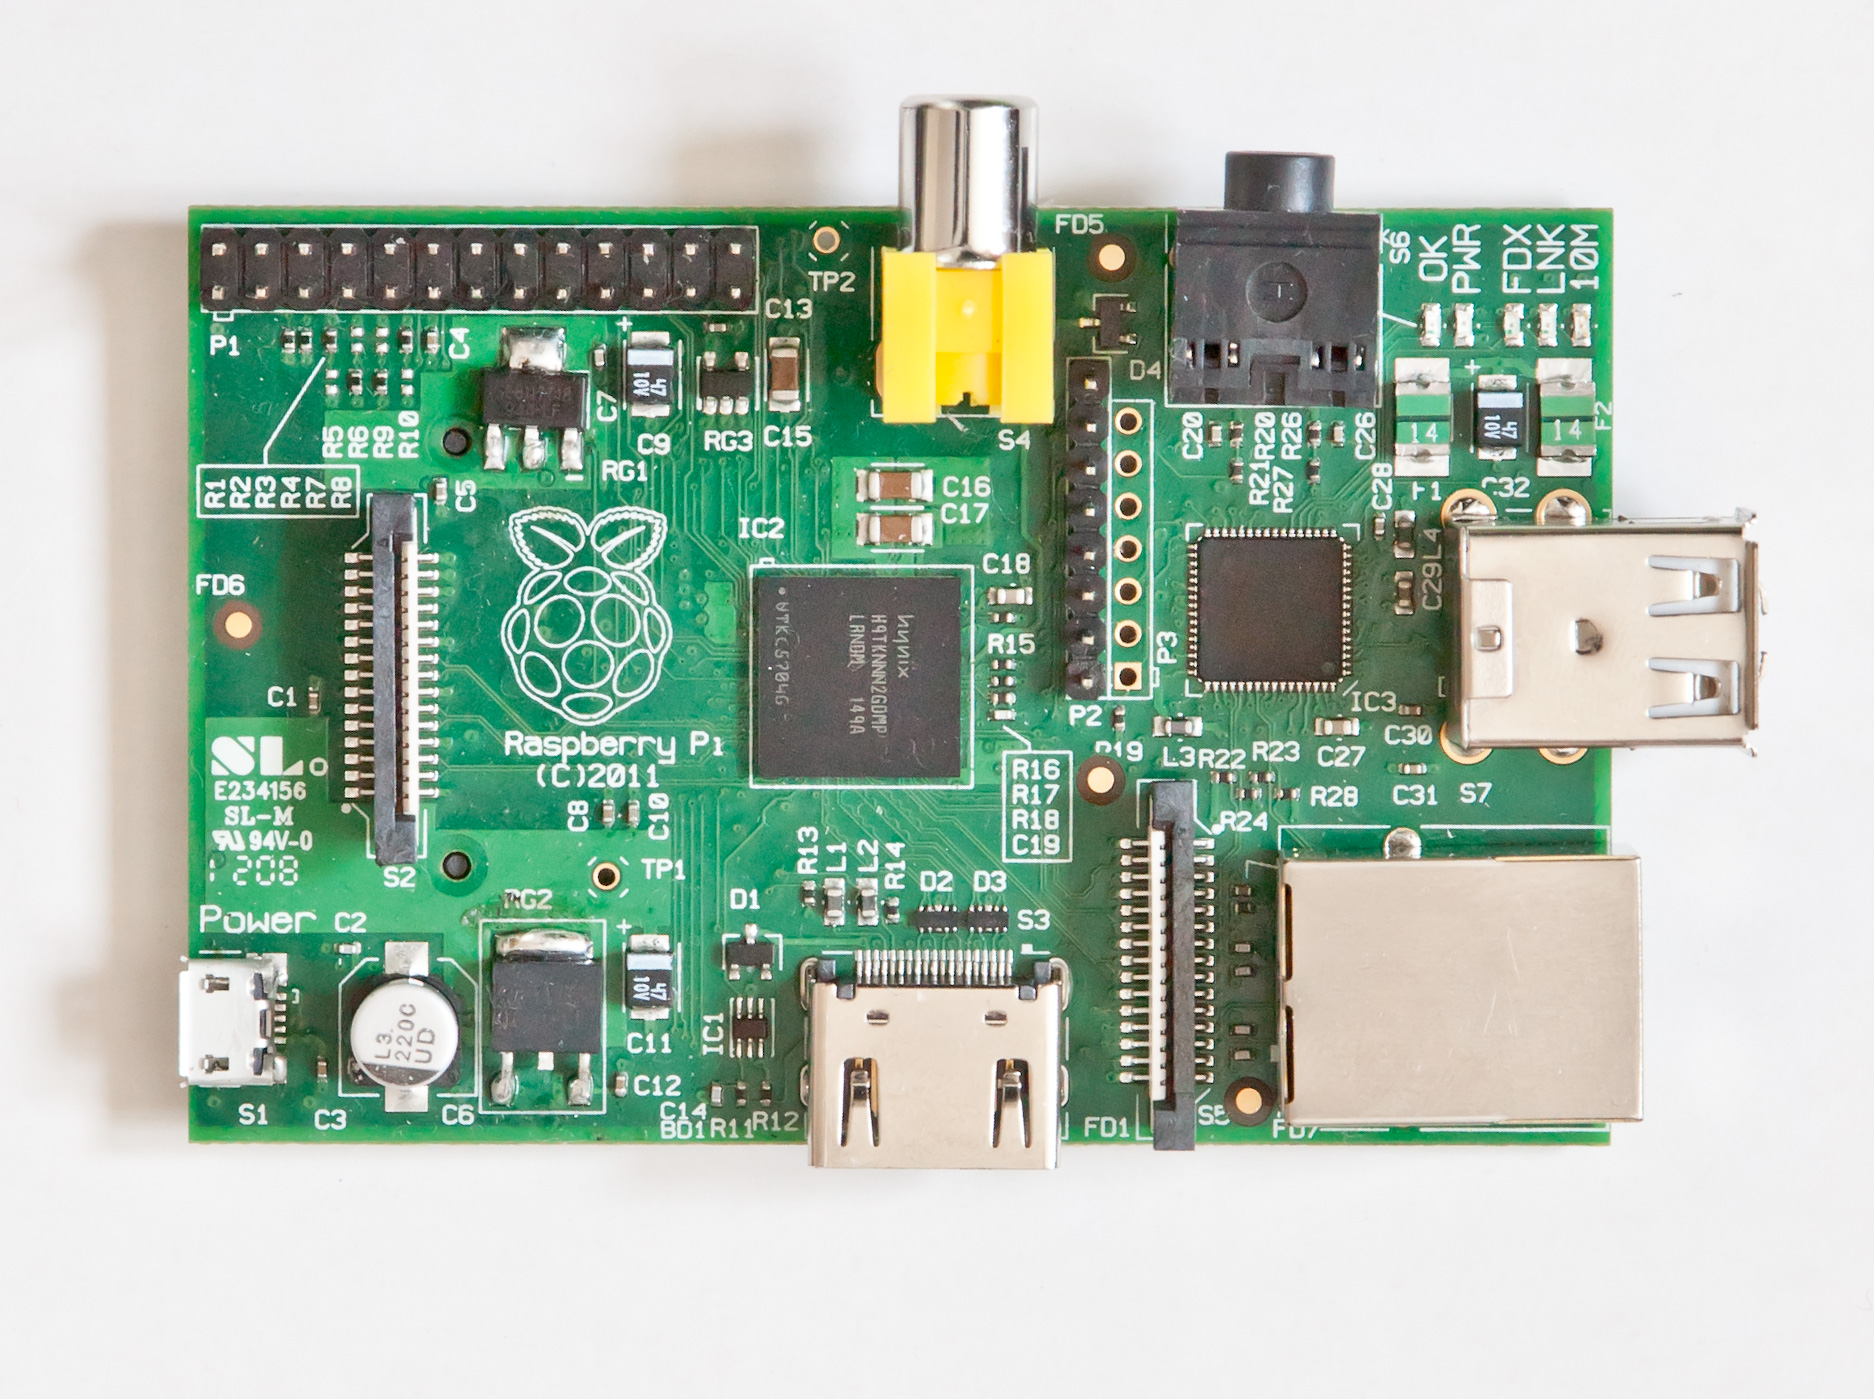
\includegraphics[scale=0.1]{Pi}
	\caption{the Raspberry Pi}\label{Pi}
\end{minipage}
\begin{minipage}[t]{0.5\textwidth}
	\centering
	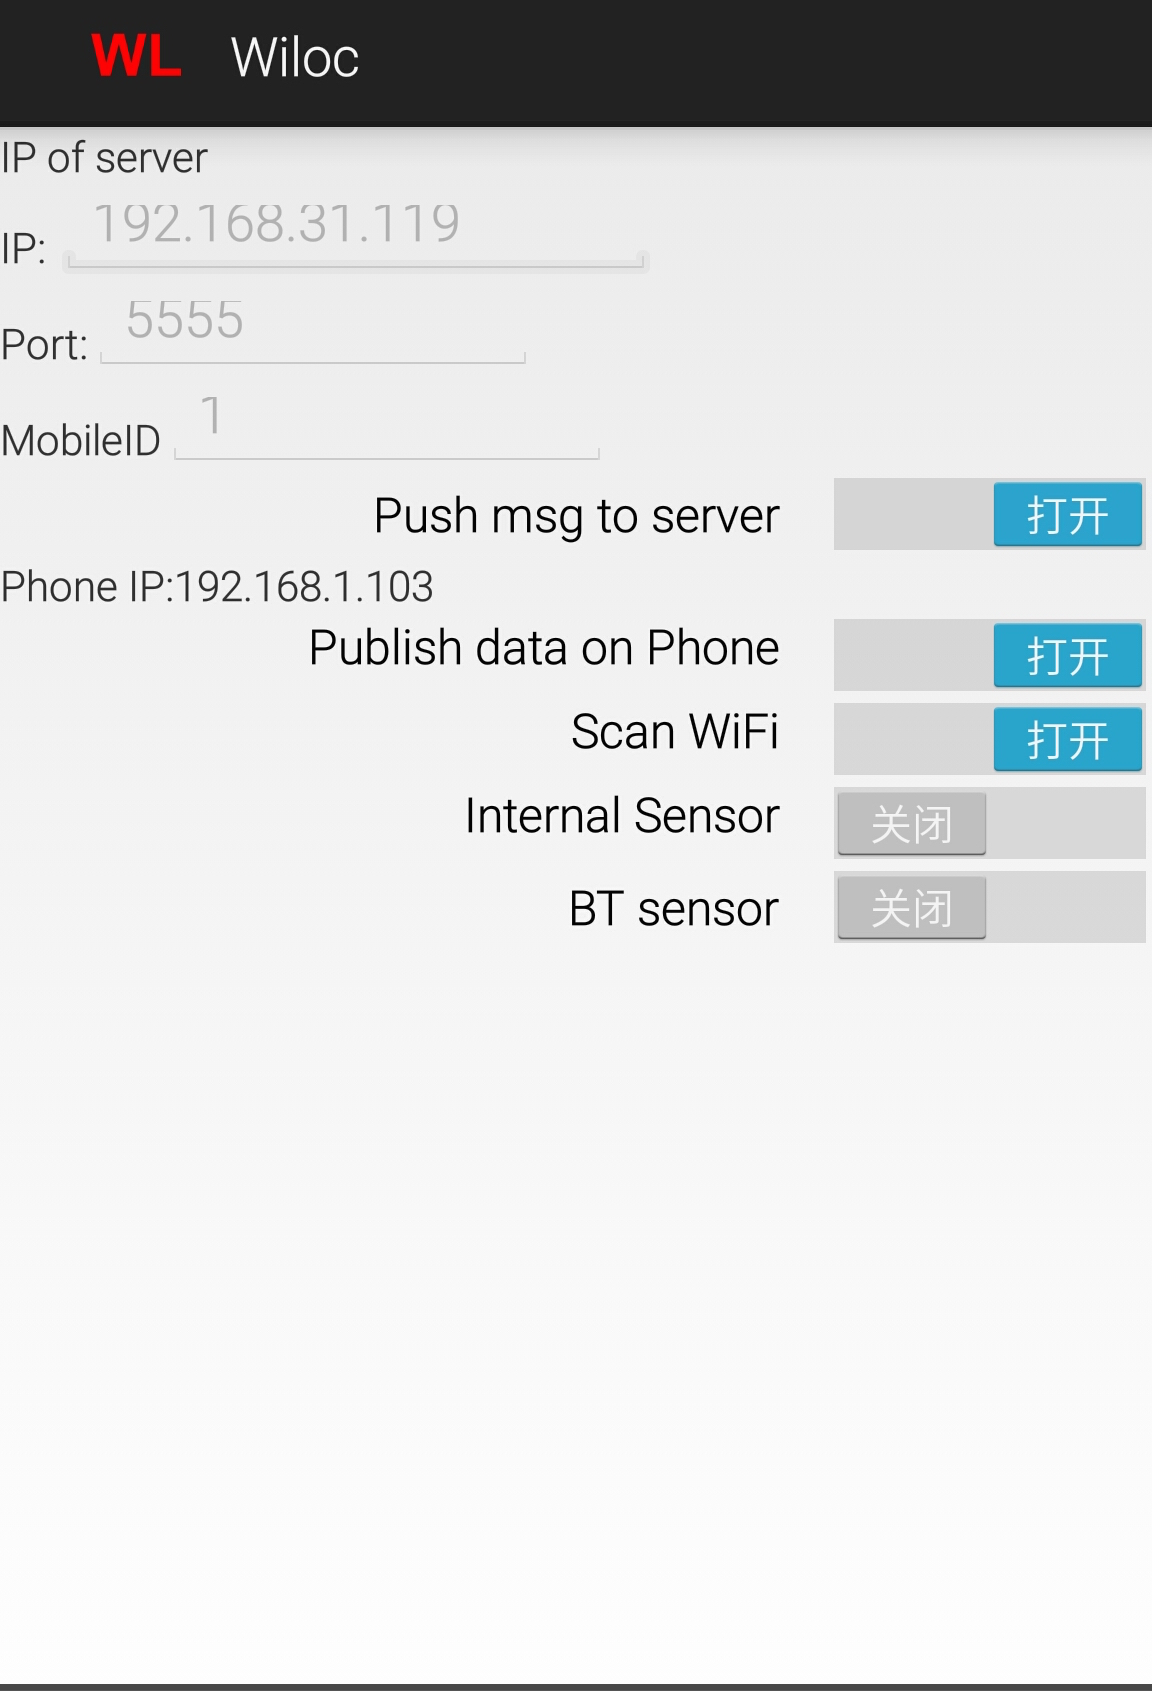
\includegraphics[scale=0.1]{app}
	\caption{Wiloclient App Interface}\label{wiloc}
\end{minipage}
\end{figure*}

%-------------------------------------------------------------------------------------------------------------------------------------
%-------------------------------------------------------------------------------------------------------------------------------------

\section{Experimental Result}
%-------------------------------------------------------------------------------------------------------------------------------------
\subsection{Path-loss and Wall Breakpoint Model}
In these models, we apply the optimal parameter values refered in \cite{site} into the models, as seen in table I. We design a Raspberry Pi layout in our experiment environments and measure the distance between Pis, then we collect RSS data to verify the models.

\begin{table}[!hbp]
\centering
\caption{Model Optimal Parameter Value}
\begin{tabular}{|c|c|}
\hline
Parameter & Optimal Value \\
\hline
$\alpha_1$ & 2 \\
\hline
$\alpha_2$ & 3.5 \\
\hline
$\alpha_E$ & 2.8 \\
\hline
$d_{bp}$ & 5 \\
\hline
$d_{wbp}$ & variable \\
\hline
$L_{0}$ & 40 \\
\hline
$L_{w}$ & 12.8 \\
\hline
\end{tabular}
\end{table}

In our system, we measured $d_{wbp}=5m$. \\
\subsubsection{Path-loss Model}
In the path-loss model verification, we substitute the distance in the model to obtain the measured path-loss value, calculate the truly path-loss value with RSS. The distance between transmitt Pis and receiver Pis ranges from $2m$ to $8m$, $d_{bp}$ just lies between the range, we can see from Fig. \ref{pathloss} that the peak diff value all lies between $35-50dB$, but as the distance grows, the number of bigger value tends to be more, even apprears $60dB$,which means as distance grows the model gradually becomes rough thus error grows.

\begin{figure*}[htbp]
\centering
\begin{minipage}[t]{0.2\textwidth}
	\centering
	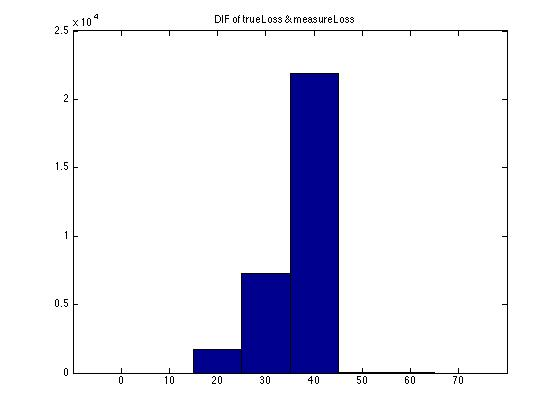
\includegraphics[scale=0.2]{pathloss0-1}
	%\caption{Pi RSS hist value as time length grows in day 1}
\end{minipage}
\begin{minipage}[t]{0.2\textwidth}
	\centering
	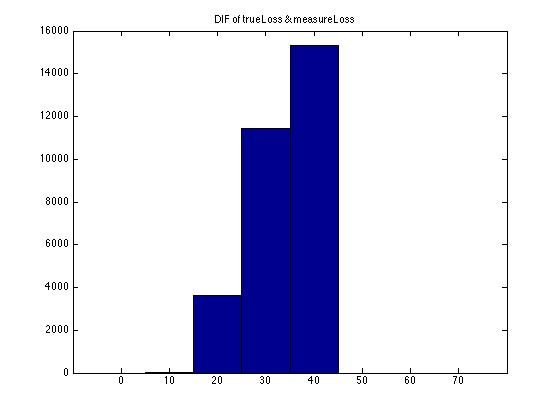
\includegraphics[scale=0.2]{pathloss0-2}
	%\caption{Pi RSS hist value as time length grows in day 2}
\end{minipage}
\begin{minipage}[t]{0.2\textwidth}
	\centering
	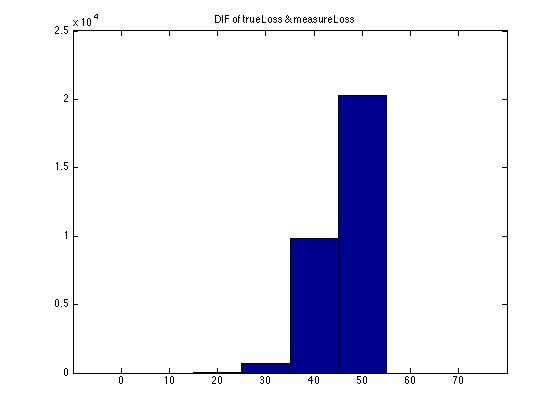
\includegraphics[scale=0.2]{pathloss0-3}
	%\caption{Pi RSS hist value as time length grows in day 3}
\end{minipage}
\begin{minipage}[t]{0.2\textwidth}
	\centering
	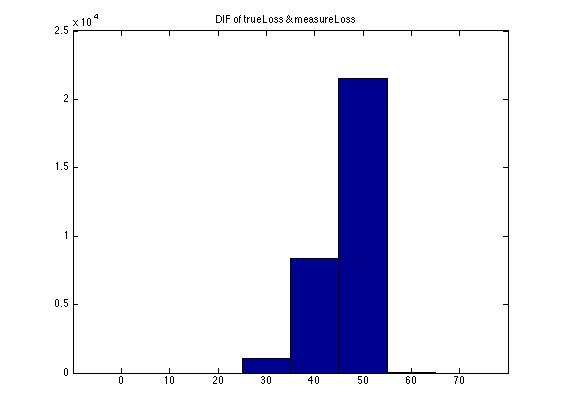
\includegraphics[scale=0.2]{pathloss0-4}
	%\caption{Pi RSS hist value as time length grows in day 4}
\end{minipage}
\caption{Path-loss Model: Diff of trueLoss and measureLoss, 4 Pi in different distance detected by Pi 1}\label{pathloss}
\end{figure*}

\subsubsection{Wall Breakpoint Model}
Wall Breakpoint Model is a bit complex as we have to consider wall factor in. In this experiment, we deploy the Pis inside and outside the wall in different distance, and compare the measured and truly path-loss value similarily. Fig. \ref{wallbreakpoint} contains 4 figures, left 2 figures show the error inside the wall, and the right 2 outside the wall. We can conclude that inside the wall, as the model is more accurate, the error tends to be smaller, outside the wall, error grows bigger and bigger error diff value appears because of the wall factor, which means the wall breakpoint model is more accurate than pass loss model, but as distances grows outside the wall, the error still grows and model also gradually becomes rough.

\begin{figure*}[htbp]
\centering
\begin{minipage}[t]{0.2\textwidth}
	\centering
	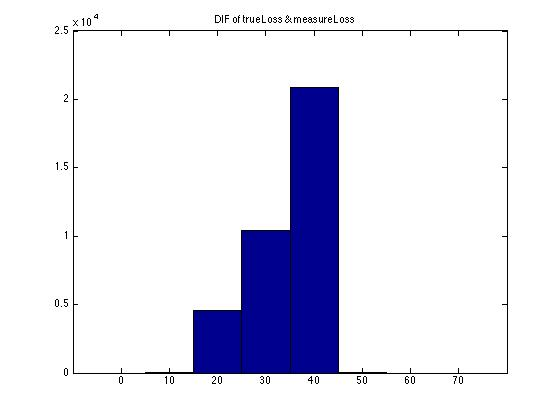
\includegraphics[scale=0.2]{wallbreakpoint0-1}
	%\caption{Pi RSS hist value as time length grows in day 1}
\end{minipage}
\begin{minipage}[t]{0.2\textwidth}
	\centering
	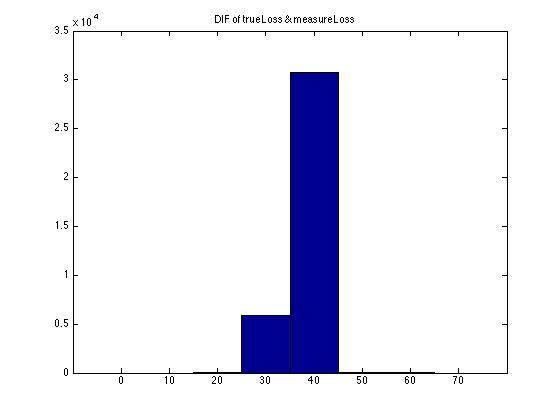
\includegraphics[scale=0.2]{wallbreakpoint0-2}
	%\caption{Pi RSS hist value as time length grows in day 2}
\end{minipage}
\begin{minipage}[t]{0.2\textwidth}
	\centering
	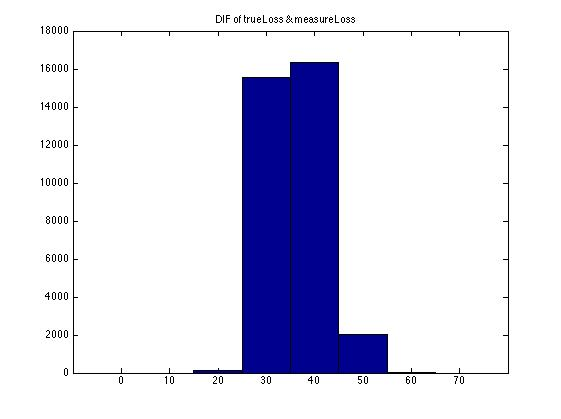
\includegraphics[scale=0.2]{wallbreakpoint0-3}
	%\caption{Pi RSS hist value as time length grows in day 3}
\end{minipage}
\begin{minipage}[t]{0.2\textwidth}
	\centering
	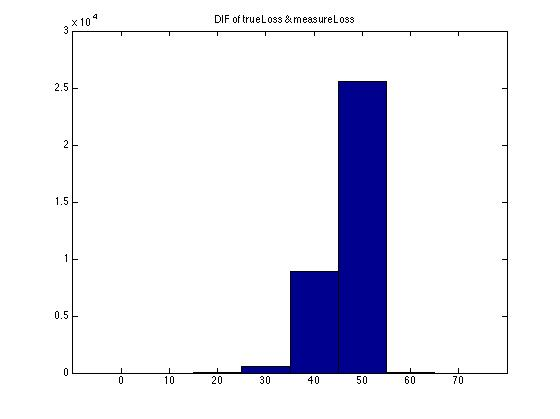
\includegraphics[scale=0.2]{wallbreakpoint0-4}
	%\caption{Pi RSS hist value as time length grows in day 4}
\end{minipage}
\caption{Wall Breakpoint Model: Diff of trueLoss and measureLoss, 4 Pi in different distance detected by Pi 1}\label{wallbreakpoint}
\end{figure*}

%-------------------------------------------------------------------------------------------------------------------------------------
\subsection{RSS variation}
RSS value is not stable, affected by envrionmental changes, that's the reason why linear regression model cannot adapt to. Therefore, before model verification, we compare and research RSS changes via different time, location and device.

%-------------------------------------------------------------------------------------------------------------------------------------

\subsubsection{RSS changes via time}
In this experiment, we choose 5 Raspberry Pis to collect data. Fig. \ref{hist} shows RSS histogram value detected by Pi 1 in 4 days, if we compare the same row in each subfigure, which means the same Pi RSS values in 4 days, we can find the distribution is not similar each day, among these Pis, some do not change anything, which means the environment would affect RSS values.
If we compare each row in one subfigure, we can see that the Pis' rss peak value appears in different position, this is reasonable, because of the Raspberry Pi lay out. The distance between detected Pi and detecting ID decides the RSS histogram value distribution. If distance between detected Pi and detecting ID is smaller, the peak value tends to bigger, vice versa. Besides, although the peak values are different, the distribution law tends to be similar. This is also reasonable, since the Raspberry Pis are actually "same", the only difference is MAC Addr, ID and distance, and they are detected by same Raspberry Pi.

Fig. \ref{hist2} shows Pi 2's RSS value distribution in different time length in 4 days. We cut the time length into 4 pieces, $\dfrac{1}{4},\dfrac{2}{4}, \dfrac{3}{4}, \dfrac{4}{4}$. The figure shows that as time length grows, the distribution law tends to be similar.



%------------------------------------------------------------------------------------------------------------------------------------------------

\subsubsection{RSS changes via block effect}
Indoor environment also affects RSS values. The first subfigure in Fig. \ref{hist} and Fig. \ref{hist2} is different from other subfigures, because the Pi's(ID=2) environment is a bit different from others, there is more block near it at that day, such as plot plant and door, thus reducing the RSS value and change the histogram distribution.
Comparing Fig. \ref{hist2} and Fig. \ref{hist3}, Pi 2 and 3's RSS hist value, we can find Pi 3's distribution is more stable than Pi. If we cut the time length into 4 equal pieces, like Fig. \ref{hist4} and Fig. \ref{hist5}, we can also find Pi 3's distribution is more stable, but in third subfigure in Fig. \ref{hist5} we can find the last period is different from others, the explanation is that in that period, a mobile blackbord is set in that area, thus affecting the RSS value.

% ------ 4 pictures in one row -----
\begin{figure*}[htbp]
\centering
\begin{minipage}[t]{0.2\textwidth}
	\centering
	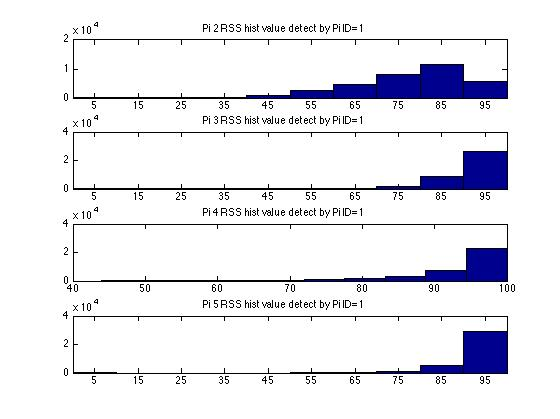
\includegraphics[scale=0.2]{time0-1}
	%\caption{Pi RSS hist value detected by same Pi in day 1}
\end{minipage}
\begin{minipage}[t]{0.2\textwidth}
	\centering
	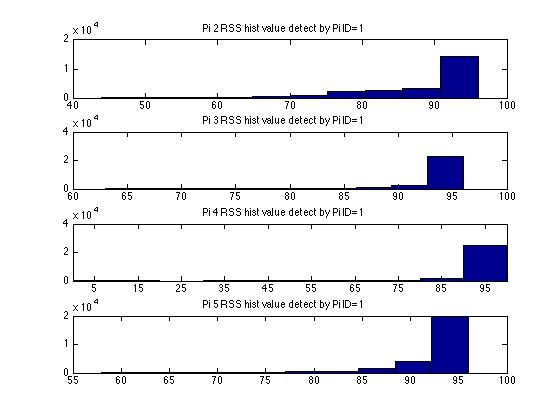
\includegraphics[scale=0.2]{time0-2}
	%\caption{Pi RSS hist value detected by same Pi in day 2}
\end{minipage}
\begin{minipage}[t]{0.2\textwidth}
	\centering
	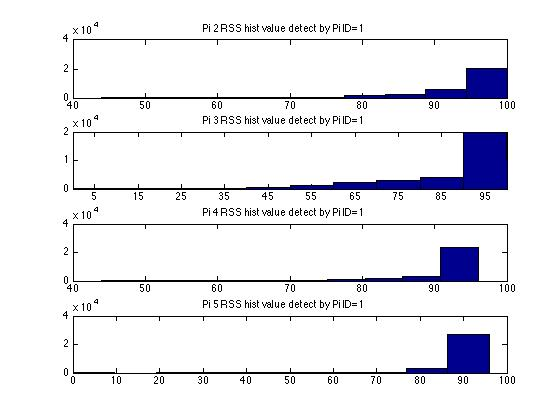
\includegraphics[scale=0.2]{time0-3}
	%\caption{Pi RSS hist value detected by same Pi in day 3}
\end{minipage}
\begin{minipage}[t]{0.2\textwidth}
	\centering
	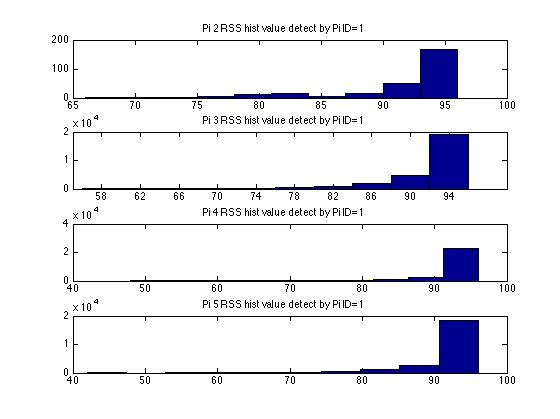
\includegraphics[scale=0.2]{time0-4}
	%\caption{Pi RSS hist value detected by same Pi in day 4}
\end{minipage}
\caption{Pi RSS hist value detected by same Pi in 4 days}\label{hist}
\end{figure*}
% ------ 4 pictures in one row -----

%----------------------------------------------1/4, 2/4, 3/4, 4/4 length---------------------------------------------------------------

\begin{figure*}[htbp]
\centering
\begin{minipage}[t]{0.2\textwidth}
	\centering
	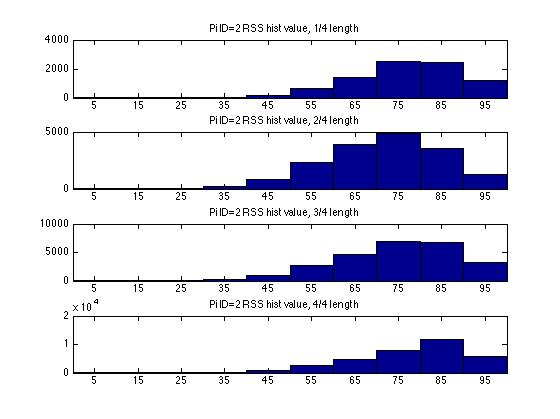
\includegraphics[scale=0.2]{time1-1}
	%\caption{Pi RSS hist value as time length grows in day 1}
\end{minipage}
\begin{minipage}[t]{0.2\textwidth}
	\centering
	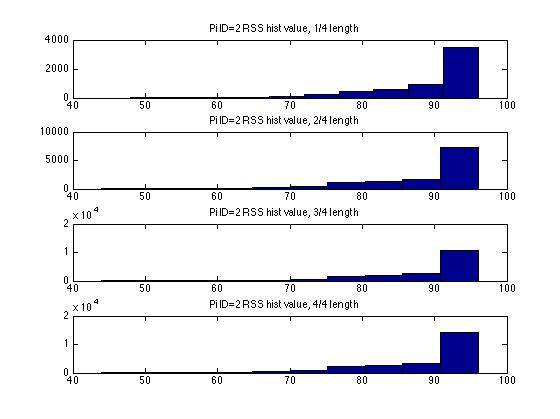
\includegraphics[scale=0.2]{time1-2}
	%\caption{Pi RSS hist value as time length grows in day 2}
\end{minipage}
\begin{minipage}[t]{0.2\textwidth}
	\centering
	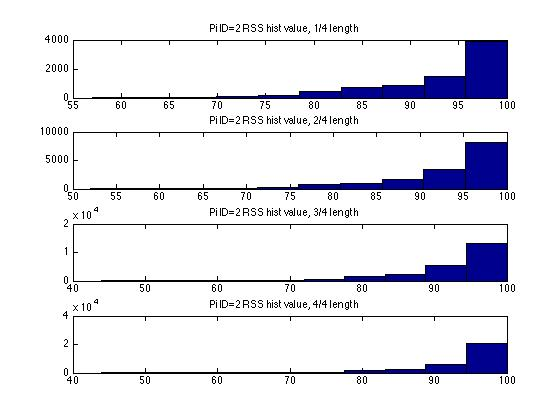
\includegraphics[scale=0.2]{time1-3}
	%\caption{Pi RSS hist value as time length grows in day 3}
\end{minipage}
\begin{minipage}[t]{0.2\textwidth}
	\centering
	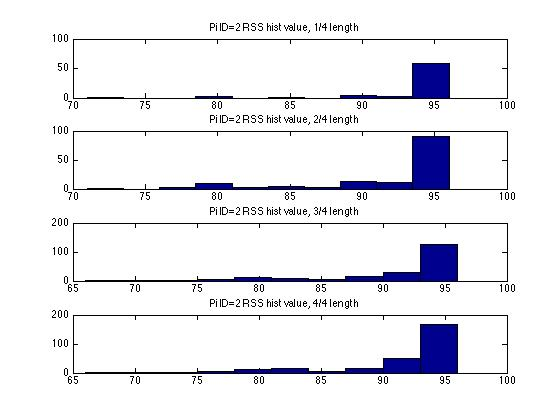
\includegraphics[scale=0.2]{time1-4}
	%\caption{Pi RSS hist value as time length grows in day 4}
\end{minipage}
\caption{Pi ID=2 RSS hist value as time length grows($\dfrac{1}{4}$,$\dfrac{2}{4}$,$\dfrac{3}{4}$,$\dfrac{4}{4}$ length) in 4 days}\label{hist2}
\end{figure*}

\begin{figure*}[htbp]
\centering
\begin{minipage}[t]{0.2\textwidth}
	\centering
	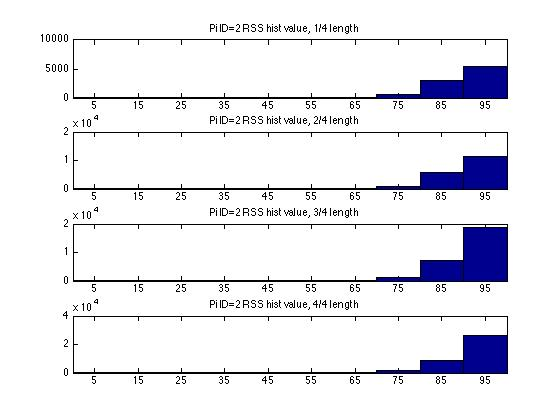
\includegraphics[scale=0.2]{time1-5}
	%\caption{Pi RSS hist value as time length grows in day 1}
\end{minipage}
\begin{minipage}[t]{0.2\textwidth}
	\centering
	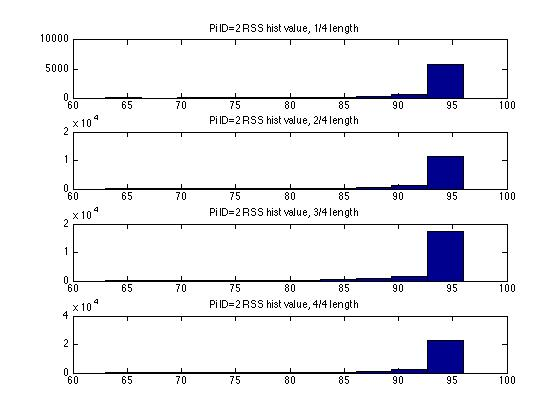
\includegraphics[scale=0.2]{time1-6}
	%\caption{Pi RSS hist value as time length grows in day 2}
\end{minipage}
\begin{minipage}[t]{0.2\textwidth}
	\centering
	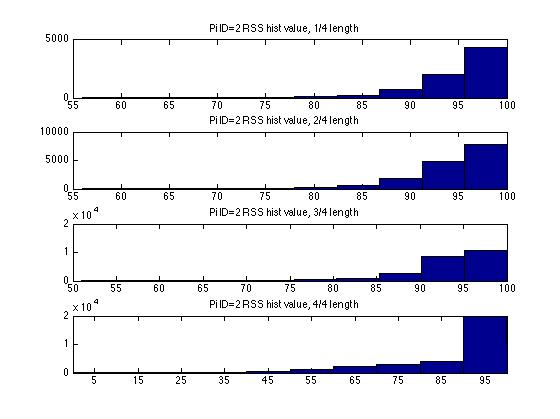
\includegraphics[scale=0.2]{time1-7}
	%\caption{Pi RSS hist value as time length grows in day 3}
\end{minipage}
\begin{minipage}[t]{0.2\textwidth}
	\centering
	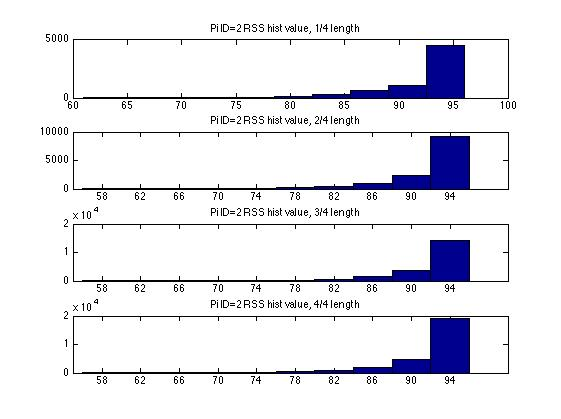
\includegraphics[scale=0.2]{time1-8}
	%\caption{Pi RSS hist value as time length grows in day 4}
\end{minipage}
\caption{Pi ID=3 RSS hist value as time length grows($\dfrac{1}{4}$,$\dfrac{2}{4}$,$\dfrac{3}{4}$,$\dfrac{4}{4}$ length) in 4 days}\label{hist3}
\end{figure*}

%-----------------------------------------------0-1/4,1/4-2/4,2/4-3/4,3/4-4/4 length ---------------------------------------------------------------
\begin{figure*}[htbp]
\centering
\begin{minipage}[t]{0.2\textwidth}
	\centering
	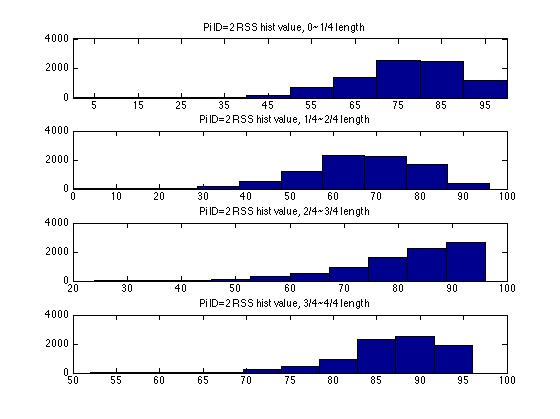
\includegraphics[scale=0.2]{time2-1}
	%\caption{Pi RSS hist value as time length grows in day 1}
\end{minipage}
\begin{minipage}[t]{0.2\textwidth}
	\centering
	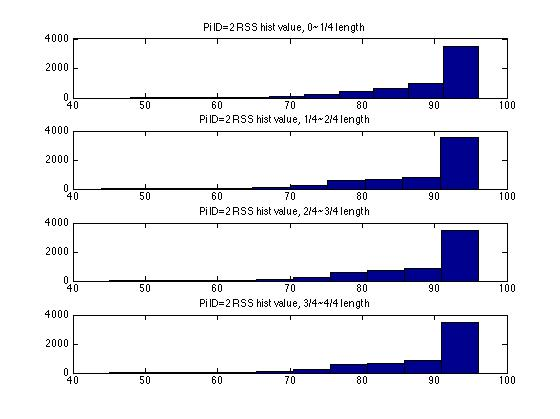
\includegraphics[scale=0.2]{time2-2}
	%\caption{Pi RSS hist value as time length grows in day 2}
\end{minipage}
\begin{minipage}[t]{0.2\textwidth}
	\centering
	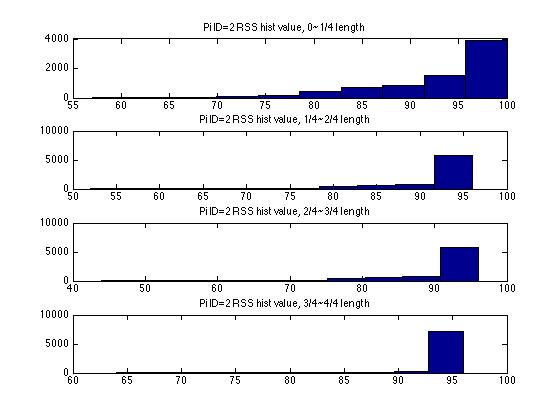
\includegraphics[scale=0.2]{time2-3}
	%\caption{Pi RSS hist value as time length grows in day 3}
\end{minipage}
\begin{minipage}[t]{0.2\textwidth}
	\centering
	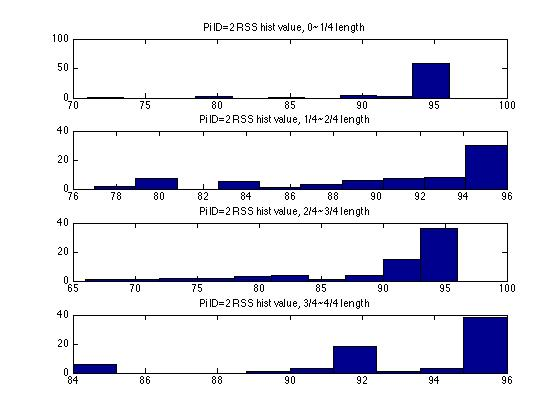
\includegraphics[scale=0.2]{time2-4}
	%\caption{Pi RSS hist value as time length grows in day 4}
\end{minipage}
\caption{Pi ID=2 RSS hist value in average time length(0-$\dfrac{1}{4}$, $\dfrac{1}{4}$-$\dfrac{2}{4}$, $\dfrac{2}{4}$-$\dfrac{3}{4}$, $\dfrac{3}{4}$-$\dfrac{4}{4}$ length) in 4 days}\label{hist4}
\end{figure*}

\begin{figure*}[htbp]
\centering
\begin{minipage}[t]{0.2\textwidth}
	\centering
	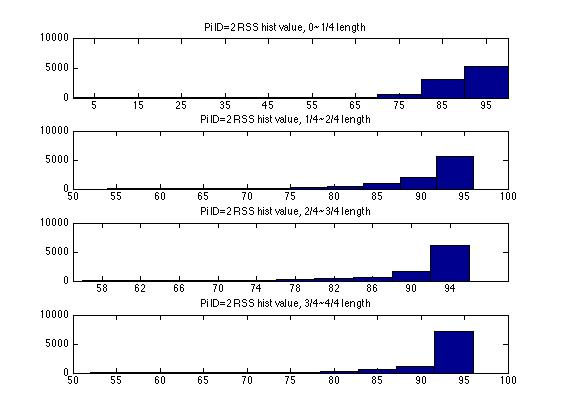
\includegraphics[scale=0.2]{time2-5}
	%\caption{Pi RSS hist value as time length grows in day 1}
\end{minipage}
\begin{minipage}[t]{0.2\textwidth}
	\centering
	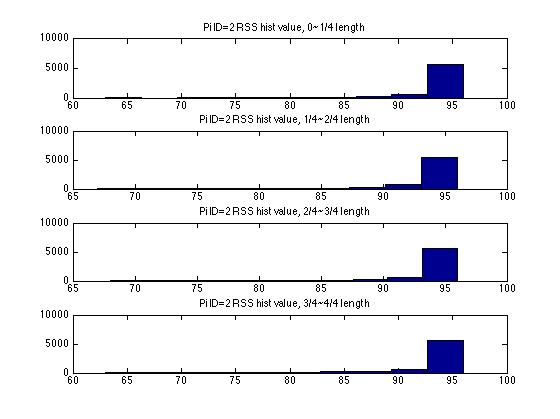
\includegraphics[scale=0.2]{time2-6}
	%\caption{Pi RSS hist value as time length grows in day 2}
\end{minipage}
\begin{minipage}[t]{0.2\textwidth}
	\centering
	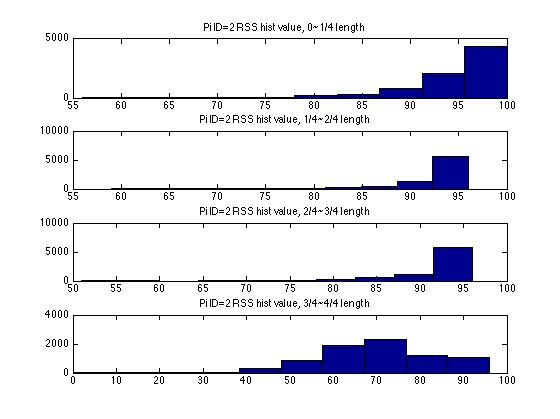
\includegraphics[scale=0.2]{time2-7}
	%\caption{Pi RSS hist value as time length grows in day 3}
\end{minipage}
\begin{minipage}[t]{0.2\textwidth}
	\centering
	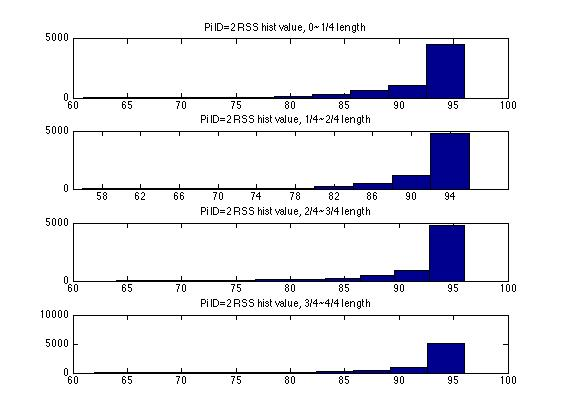
\includegraphics[scale=0.2]{time2-8}
	%\caption{Pi RSS hist value as time length grows in day 4}
\end{minipage}
\caption{Pi ID=3 RSS hist value in average time length(0-$\dfrac{1}{4}$, $\dfrac{1}{4}$-$\dfrac{2}{4}$, $\dfrac{2}{4}$-$\dfrac{3}{4}$, $\dfrac{3}{4}$-$\dfrac{4}{4}$ length) in 4 days}\label{hist5}
\end{figure*}

%------------------------------------------------------------------------------------------------------------------------------------------------

\subsubsection{RSS changes via location}
RSS also changes via location. Fig. \ref{hist6} shows Pi 1's RSS histogram value detected by other 4 pis in 4 days. Each subfigure shows Pi 2~5's detection from Pi 1, we can see that as the distance between Pi 2~5 and Pi 1 is different, RSS values are different, which menas location affects RSS values. Besides, if we compare the same row in each subfigure, we can see difference, which also verifies that envrionment changes affect RSS value. 

\begin{figure*}[htbp]
\centering
\begin{minipage}[t]{0.2\textwidth}
	\centering
	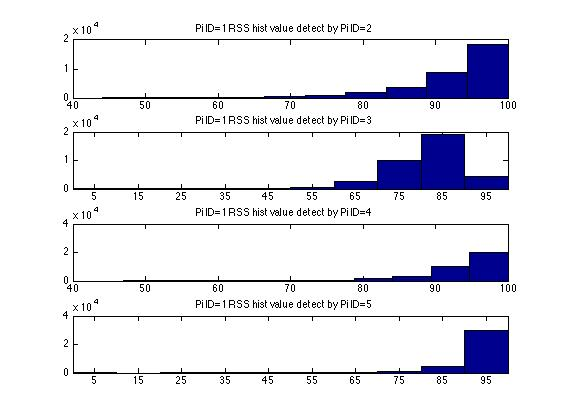
\includegraphics[scale=0.2]{location0-1}
	%\caption{Pi RSS hist value detected by same Pi in day 1}
\end{minipage}
\begin{minipage}[t]{0.2\textwidth}
	\centering
	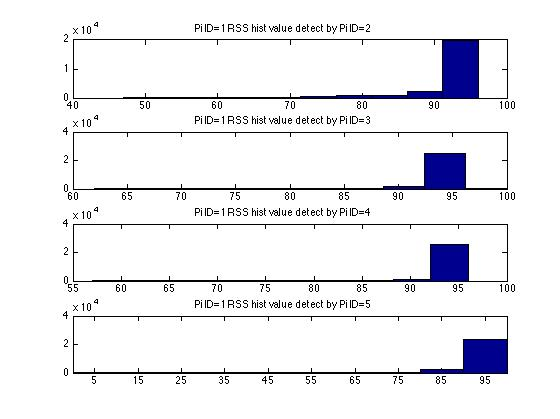
\includegraphics[scale=0.2]{location0-2}
	%\caption{Pi RSS hist value detected by same Pi in day 2}
\end{minipage}
\begin{minipage}[t]{0.2\textwidth}
	\centering
	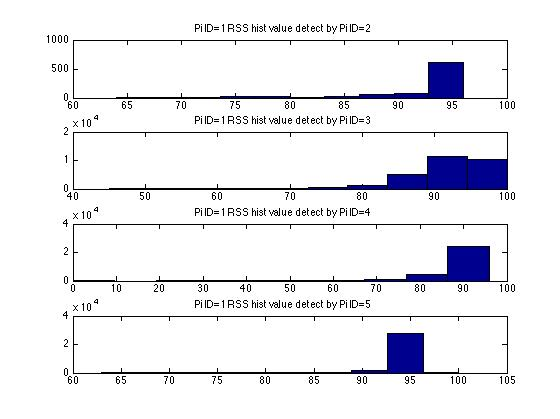
\includegraphics[scale=0.2]{location0-3}
	%\caption{Pi RSS hist value detected by same Pi in day 3}
\end{minipage}
\begin{minipage}[t]{0.2\textwidth}
	\centering
	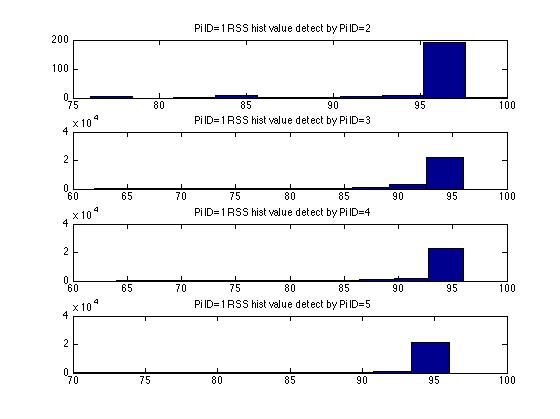
\includegraphics[scale=0.2]{location0-4}
	%\caption{Pi RSS hist value detected by same Pi in day 4}
\end{minipage}
\caption{Pi 1's RSS hist value detected by other 4 Pis in 4 days}\label{hist6}
\end{figure*}


%-------------------------------------------------------------------------------------------------------------------------------------

\subsubsection{RSS changes via different devices}
The Raspberry Pi and mobile device can both detect AP RSS around, to verify the device impact on RSS, we choose serveral Raspberry Pis and mobile devices (mainly Nexus 5 and Tablet, installed with \textit{Wiloclient}) as the experimental devices. We fix one Raspberry Pi and a mobile device together as a "group", which means they are in the same location and environment, and allocate the groups in different locations, by comparing the RSS detected by the "group" we can find out the device impact on RSS. We compare the RSS detected by Raspberry Pi and mobile device in same group, the RSS contains serveral locations, so we can check more than one place.
Fig. \ref{hist7} shows 3 Pi's histogram value detected by Pi 1 and mobile device. Each subfigure represents one Pi's detection. The result shows different devices also affect RSS values.
Fig. \ref{errorbar} shows the growing and average sequence errorbar. Each subfigure represents one Raspberry Pi's RSS errorbar detected by mobile device.

\begin{figure*}[htbp]
\centering
\begin{minipage}[t]{0.2\textwidth}
	\centering
	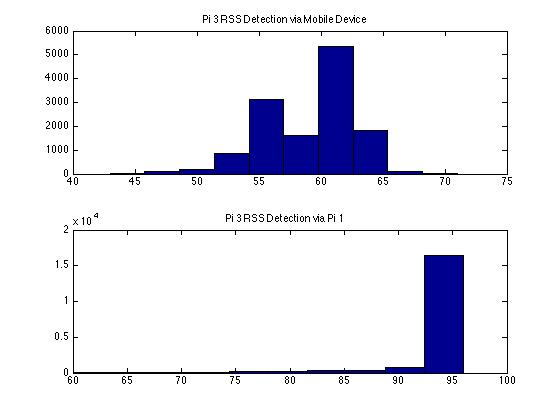
\includegraphics[scale=0.2]{device0-1}
	%\caption{Pi RSS hist value detected by same Pi in day 1}
\end{minipage}
\begin{minipage}[t]{0.2\textwidth}
	\centering
	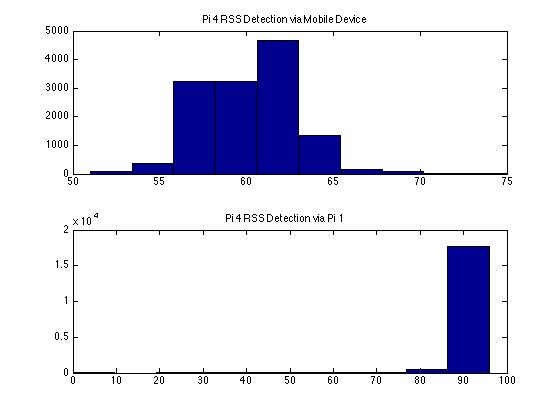
\includegraphics[scale=0.2]{device0-2}
	%\caption{Pi RSS hist value detected by same Pi in day 2}
\end{minipage}
\begin{minipage}[t]{0.2\textwidth}
	\centering
	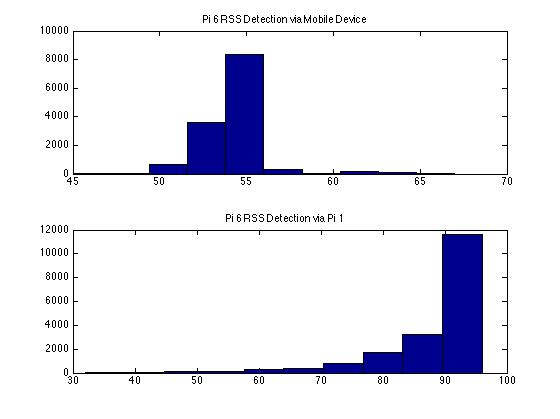
\includegraphics[scale=0.2]{device0-3}
	%\caption{Pi RSS hist value detected by same Pi in day 3}
\end{minipage}
%\begin{minipage}[t]{0.2\textwidth}
%	\centering
%	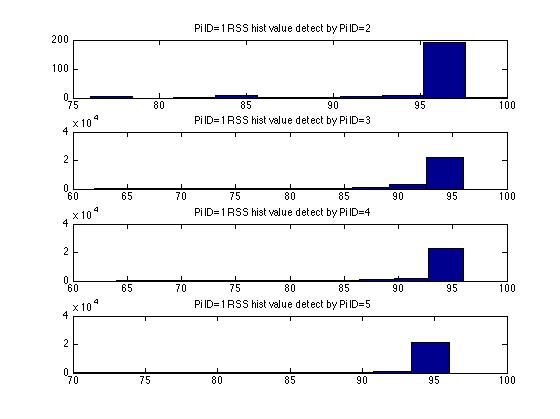
\includegraphics[scale=0.2]{location0-4}
	%\caption{Pi RSS hist value detected by same Pi in day 4}
%\end{minipage}
\caption{3 Pi RSS hist value via Pi 1 and mobile device}\label{hist7}
\end{figure*}

% ------ two pictures in one row -----
\begin{figure*}[htbp]
%\centering
\begin{minipage}[t]{0.5\textwidth}
	\centering
	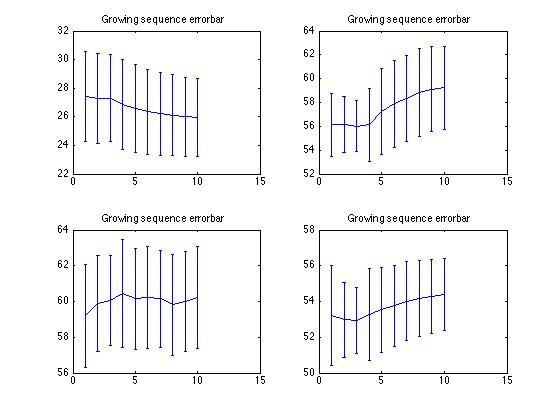
\includegraphics[scale=0.5]{device1-1}
	%\caption{whole sequence}
\end{minipage}
\begin{minipage}[t]{0.5\textwidth}
	\centering
	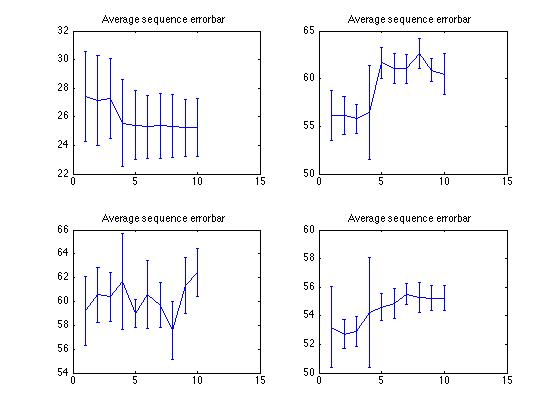
\includegraphics[scale=0.5]{device1-2}
	%\caption{after mean}
\end{minipage}
\caption{Growing and Average sequence errorbar}\label{errorbar}
\end{figure*}
% ------ two pictures in one row -----

%-------------------------------------------------------------------------------------------------------------------------------------

\subsection{Inter-Raspberry Pi Model Verification}
We collect 5 days' data continuously, each day data could be considered as an independent data set, named $A,B,C,D,E$. We use each as offline training set and others as online verification set, and calculate the SRE. The result is shown as Table \ref{interModel} : \\

\begin{table}[!hbp]
\centering
\begin{tabular}{|c|c|c|c|c|c|}
    	\hline
	SRE & A & B & C & D & E \\
	\hline
	A & *31.6139* & 73.9588 & 51.8962 &101.3744 & 74.1551 \\
    	\hline
	B & 71.7112 & *38.2634* & 79.9411 & 90.2935 & 108.8354 \\
    	\hline
	C & 46.6203 & 80.5898 & *38.7940* & 99.3180 & 59.0646 \\
	\hline
	D & 114.1456 & 107.9651 & 96.5616 & *41.5062* & 107.8099 \\
	\hline
	E & 58.2869 & 99.6614 & 56.0502 &128.6478 & *26.6933* \\
	\hline
\end{tabular}
\caption{Inter-Raspberry Pi Model Verification SRE Value}\label{interModel}
\end{table}

The diagonal elements means the least square method error, that is, we use offline same data to compare with calculated data. Other elements show the actua error, for example, 73.9588, is the error calculated with data set $A$ as offline training set, data set $B$ as online verification set.
We can see the environmental change impacts' on model from the data. The error becomes large and thus offline training coefficients become out-of-date.

%-------------------------------------------------------------------------------------------------------------------------------------

\subsection{Radiomap Model Verification}
Same as inter-Raspberry Pi model, we collect data continuously as independent data set every day, the result is shown as Table \ref{radiomapModel}: \\

\begin{table}[!hbp]
\centering
\begin{tabular}{|c|c|c|c|c|c|}
    	\hline
	SRE & A & B & C & D & E \\
	\hline
	A & *9.3023* & 25.9349 & 31.3394 & 26.6844 & 20.4334 \\
    	\hline
	B & 27.3431 & *5.6803* & 16.8809 & 15.6774 & 12.5918 \\
    	\hline
	C & 29.3644 & 17.3275 & *7.6845* & 15.1264 & 13.7434 \\
	\hline
	D & 20.0525 & 15.1599 & 14.1721 & *7.1387* & 16.7880 \\
	\hline
	E & 24.5801 & 12.2351 & 15.9936 & 17.5971 & *5.5749* \\
	\hline
\end{tabular}
\caption{Radiomap Model Verification SRE Value}\label{radiomapModel}
\end{table}

The calculated error sheet further verifies the environmental changes' impact on model.
%-------------------------------------------------------------------------------------------------------------------------------------

\section{Conclusion and Future Work}
In this paper, we build a novel system to verify two popular indoor positioning models: radio channel model and linear regression model. We introduce a cheap and easy to configure hardware called Raspberry Pi act as wlan AP, it can be both transmitter and receiver and automatically send data to server after configuration. In radio channel area, we consider path-loss and wall breakpoint model, the results show that the model is not that robust. In linear regression area, we discuss inter-Raspberry Pi and radiomap model, the result shows that environmental change impact on fingerprint linear regression model matters much, which makes the offline training out-of-date. \yc{Finally, we put forward a novel online adaptive algorithm to solve the parameter outdating problem, the simulation shows good results. The online adaptive method leaves offline training alone, which means reducing much offline calculating time, while solves the environmental changes impact problem... } In the future, work should focus on optimizing the \textit{NormScore} algorithm, and simulate online adaptive algorithm in real environment to verify the accuracy on indoor positioning.
%-------------------------------------------------------------------------------------------------------------------------------------

%References, \bibitem{citename}, using in text: \cite{citename}
\begin{thebibliography}{1}

\bibitem{radar} P. Bahl, V.N. Padmanabhan {\em RADAR: an in-building RF-based user location and tracking system, in}: Proc. of IEEE INFOCOM, 2000.

\bibitem{site} B.Roberts, Kaveh Pahlavan {\em Site-specific rss signature modeling for WiFi localization}: Proc. of IEEE GLOBECOM, 2009.

\bibitem{dynamic} M. Atia, A. Noureldin and M. Korenberg {\em Dynamic online-calibrated radio maps for indoor positioning in wireless local area networks}: IEEE TMC, VOL. 12, NO. 9, 2013

\bibitem{wireless} K. Pahlavan and A. Levesque {\em Wireless Information Networks}: John Wiley and Sons, 1995.

\bibitem{raspberry} Raspberry Pi {\em www.raspberrypi.org}

\bibitem{zmq} Zeromq Protocol {\em www.zeromq.org}

\end{thebibliography}

\end{document}